\documentclass[aspectratio=169,10pt]{beamer}
\usetheme[progressbar=frametitle,sectionpage=progressbar]{metropolis}
\usepackage{amsmath,amssymb,bm,booktabs,graphicx}
\usepackage{tikz}
\usetikzlibrary{arrows.meta,decorations.pathreplacing,calc}

\newcommand{\um}{\,\mu\mathrm{m}}
\newcommand{\J}{\mathcal{J}}
\newcommand{\A}{\mathsf{A}}
\newcommand{\N}{\mathbf{N}}
\newcommand{\Fin}{F_{\mathrm{in}}}
\newcommand{\rdet}{r_{\mathrm{det}}}
\newcommand{\Cstk}{C_{\mathrm{stk}}}
\definecolor{askcol}{HTML}{C0392B}
\newcommand{\ask}[1]{\textcolor{askcol}{\textbf{#1}}}

\title{Estimating turbulent broadening of cloud droplet size distributions}
\subtitle{Recovering an effective diffusivity $D_x$ from droplet-size histograms}
\author{Dawson Collins}
\institute{Brigham Young University}
\date{October 2026}

\graphicspath{{figures/}}

\begin{document}
\maketitle

%==================================================================
\section{The problem}
%==================================================================

\begin{frame}{Why droplet size distributions matter}
\begin{columns}[c]
\begin{column}{0.56\textwidth}
\begin{itemize}\small
\item The \textbf{width} of the droplet size distribution (DSD) controls how often droplets collide, and so when drizzle forms
\item \textbf{Turbulence broadens the DSD}: droplets wander through moister and drier air and grow at different rates
\item \textbf{Pi Chamber} (MTU): a steady turbulent cloud. Aerosol is injected, activates, grows, and falls out
\item Clean clouds (few droplets) have broader DSDs than polluted ones (Chandrakar et al.\ 2016, 2018)
\end{itemize}
\vspace{0.3em}
\textbf{Question:} how strong is the turbulent broadening, and can we infer it from measured DSDs?
\end{column}
\begin{column}{0.42\textwidth}
\centering
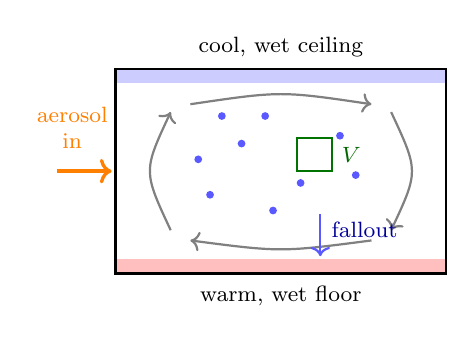
\begin{tikzpicture}[x=1cm,y=1cm,font=\footnotesize]
\fill[red!25] (0,0) rectangle (4.2,0.18);
\fill[blue!20] (0,2.42) rectangle (4.2,2.6);
\draw[thick] (0,0) rectangle (4.2,2.6);
\node at (2.1,-0.28) {warm, wet floor};
\node at (2.1,2.88) {cool, wet ceiling};
\draw[->,thick,gray] (0.7,0.55) .. controls (0.35,1.3) .. (0.7,2.05);
\draw[->,thick,gray] (0.95,2.15) .. controls (2.1,2.32) .. (3.25,2.15);
\draw[->,thick,gray] (3.5,2.05) .. controls (3.85,1.3) .. (3.5,0.55);
\draw[->,thick,gray] (3.25,0.42) .. controls (2.1,0.27) .. (0.95,0.42);
\foreach \p in {(1.2,1.0),(1.6,1.65),(2.35,1.15),(2.85,1.75),(2.0,0.8),(1.35,2.0),(3.05,1.25),(1.9,2.0),(1.05,1.45)}
  \fill[blue!65] \p circle (1.4pt);
\draw[->,very thick,orange] (-0.75,1.3) -- (-0.05,1.3);
\node[orange,align=center] at (-0.55,1.85) {aerosol\\in};
\draw[thick,green!45!black] (2.3,1.3) rectangle (2.75,1.72);
\node[green!40!black,right] at (2.75,1.51) {$V$};
\draw[->,thick,blue!65] (2.6,0.75) -- (2.6,0.22);
\node[blue!60!black,right] at (2.62,0.55) {fallout};
\end{tikzpicture}\\[0.3em]
{\footnotesize Probe samples a small volume $V$.}
\end{column}
\end{columns}
\end{frame}

%------------------------------------------------------------------
\begin{frame}{Droplet growth as a random walk in $x = r^2$}
\begin{columns}[T]
\begin{column}{0.56\textwidth}
\centering
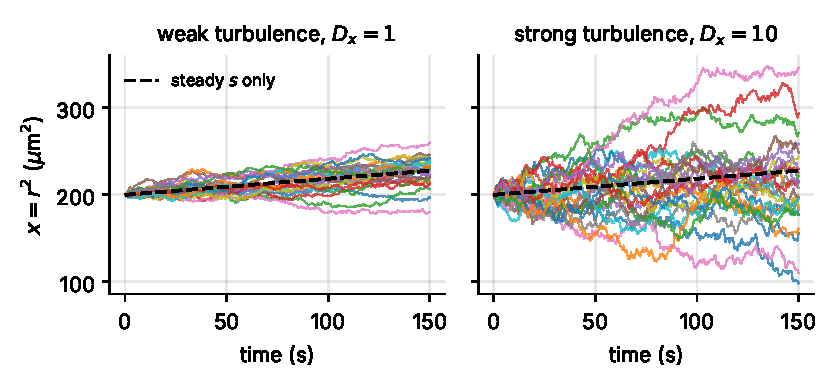
\includegraphics[width=\textwidth]{d_walks.pdf}\\
{\footnotesize 25 simulated droplets starting at the same size.}
\end{column}
\begin{column}{0.42\textwidth}
\begin{itemize}
\item Condensation: $r\,\dfrac{dr}{dt} = \xi s \;\Rightarrow\; \dfrac{d(r^2)}{dt} = a\,s$, a constant rate in $x = r^2$
\item Turbulence makes $s$ fluctuate, so growth is a random walk
\item Many droplets: \textbf{drift} (mean growth, Köhler effects) plus \textbf{diffusion} with coefficient $D_x$
\item Heuristically $D_x \approx a^2\sigma_s^2\tau_s$ (variance and correlation time of $s$ seen by a droplet)
\end{itemize}
\vspace{0.2em}
\small $D_x$ is an \emph{effective} coefficient: it absorbs any broadening the drift does not explain.
\end{column}
\end{columns}
\end{frame}

%------------------------------------------------------------------
\begin{frame}{Goal and roadmap}
\textbf{Goal:} estimate a constant $D_x$ from histograms of droplet sizes, with an honest error bar.\\[0.8em]
\textbf{A ladder of synthetic experiments}, adding one complication at a time; the true $D_x$ is known, so we can check the answers.
\begin{enumerate}
\item Steady state, exact data, only $D_x$ unknown \hfill \textbf{done}
\item Steady state, instrument-like sampled data: Poisson counts, detection limit \hfill \textbf{done}
\item Truth from a finer grid, then from a stochastic particle model \hfill next
\item Estimate the supersaturation $s$ together with $D_x$ \hfill next
\item Simulation output (C-ODT, LES, DNS), then Pi Chamber data; time dependence \hfill later
\end{enumerate}
\end{frame}

%==================================================================
\section{The forward model}
%==================================================================

\begin{frame}{The steady Fokker--Planck equation}
\begin{columns}[T]
\begin{column}{0.53\textwidth}
\[
\boxed{\frac{dF}{dx} + \lambda(x)\,N = 0,\quad F = A(x)\,N - D_x\,\frac{dN}{dx}}
\]
\begin{itemize}\small
\item $F$: flux of droplets growing past size $x$
\item Drift $A = a\,(s - A_k/r + B_k/r^3)$: condensation with Köhler curvature and salt terms
\item Fallout $\lambda = (\Cstk/h)\,x$: Stokes fall speed over chamber height
\item Injection $F(x_{\min}) = \Fin$; no flux at $r = 30\um$
\end{itemize}
\end{column}
\begin{column}{0.45\textwidth}
\textbf{What $N$ tells us}
\begin{itemize}\small
\item $N(x)\,dx$: droplets per cm$^3$ with $r^2\in[x, x+dx]$
\item Units cm$^{-3}\mu$m$^{-2}$: a \emph{density} in size, like a histogram divided by its bin width
\item Total concentration: $n = \int N\,dx$ (cm$^{-3}$)
\item Expected, chamber-averaged (not one sample)
\end{itemize}
\end{column}
\end{columns}
\vspace{0.1em}
\centering
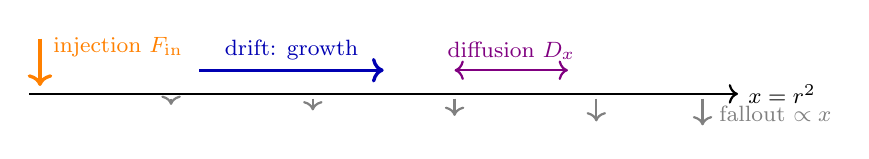
\begin{tikzpicture}[font=\footnotesize,x=0.9cm,y=1cm]
\draw[->,thick] (0,0) -- (10,0) node[right] {$x=r^2$};
\draw[->,very thick,orange] (0.15,0.7) -- (0.15,0.1); \node[orange,right] at (0.2,0.6) {injection $\Fin$};
\draw[->,very thick,blue!70!black] (2.4,0.3) -- (5.0,0.3) node[midway,above] {drift: growth};
\draw[<->,thick,violet] (6.0,0.3) -- (7.6,0.3) node[midway,above] {diffusion $D_x$};
\foreach \x/\l in {2/0.08,4/0.15,6/0.22,8/0.29,9.5/0.34} \draw[->,thick,gray] (\x,-0.06) -- (\x,-0.06-\l);
\node[gray,right] at (9.6,-0.25) {fallout $\propto x$};
\end{tikzpicture}
\end{frame}

%------------------------------------------------------------------
\begin{frame}{What the solutions look like}
\begin{columns}[c]
\begin{column}{0.5\textwidth}
\centering
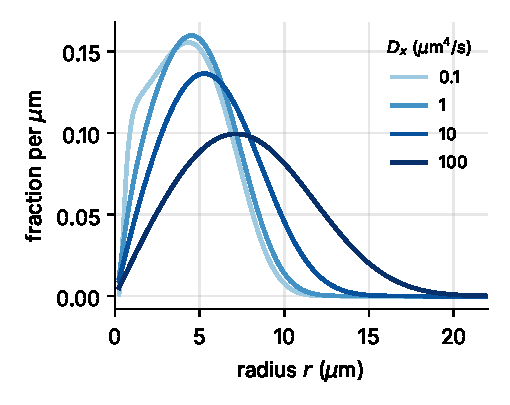
\includegraphics[width=\textwidth]{d_dsd.pdf}
\end{column}
\begin{column}{0.48\textwidth}
Larger $D_x$ gives a broader distribution, more large droplets, and fewer droplets in total (large droplets fall out quickly).\\[0.6em]
\small
\begin{tabular}{@{}rcc@{}}
\toprule
$D_x$ ($\mu$m$^4$/s) & droplets per cm$^3$ & mean radius\\\midrule
0.1 & 34{,}400 & $4.4\um$\\
1 & 29{,}900 & $4.8\um$\\
10 & 20{,}600 & $5.7\um$\\
100 & 10{,}900 & $7.9\um$\\\bottomrule
\end{tabular}\\[0.4em]
{\footnotesize $s = 0.09\%$, NaCl $r_{\rm dry}=0.065\um$, $h = 1$ m, $\Fin = 100$ cm$^{-3}$s$^{-1}$ (arbitrary scale).}
\end{column}
\end{columns}
\end{frame}

%------------------------------------------------------------------
\begin{frame}{Numerical solution}
\begin{columns}[T]
\begin{column}{0.52\textwidth}
\begin{itemize}
\item Steve's finite-volume solver, in Python: 8000 cells in $x$; $N_i$ = average of $N$ over cell $i$
\item Each cell balances flux in, flux out, and fallout (Scharfetter--Gummel fluxes, positive even when drift dominates):
\[
\A(D_x)\,\N = \mathbf{b}\quad\text{(tridiagonal)}
\]
\item Reproduces the benchmark mean radii $4.22$ and $5.74\um$ ($D_x = 0.01$, $10$)
\item \textbf{Numerical diffusion:} the scheme smears like an extra $|A|\Delta x/2\approx0.01\um^4$/s, so small $D_x$ needs $\Delta x \lesssim D_x/|A|$
\end{itemize}
\end{column}
\begin{column}{0.46\textwidth}
\centering
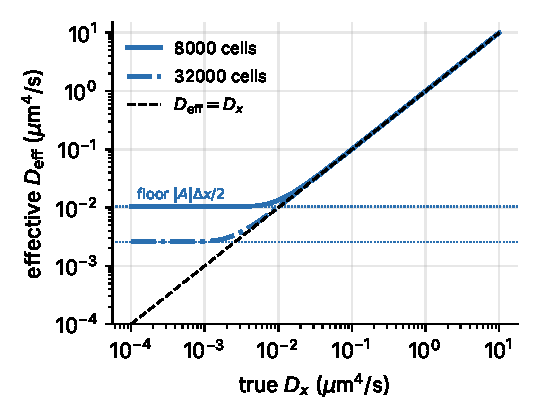
\includegraphics[width=0.95\textwidth]{d_numdiff.pdf}\\
{\footnotesize Below the floor, changing $D_x$ no longer changes the computed solution.}
\end{column}
\end{columns}
\end{frame}

%==================================================================
\section{Data and statistical model}
%==================================================================

\begin{frame}{What an instrument sees}
\begin{itemize}
\item The instrument examines a small \textbf{sample volume} $V$ of chamber air \ask{(Q1)}
\item It sorts the droplets it finds into size bins: data are \textbf{counts} $c_k$ \ask{(Q2)}
\item It cannot see droplets below a \textbf{detection limit} $\rdet$ \ask{(Q4)}
\end{itemize}
\vspace{0.2em}
\centering
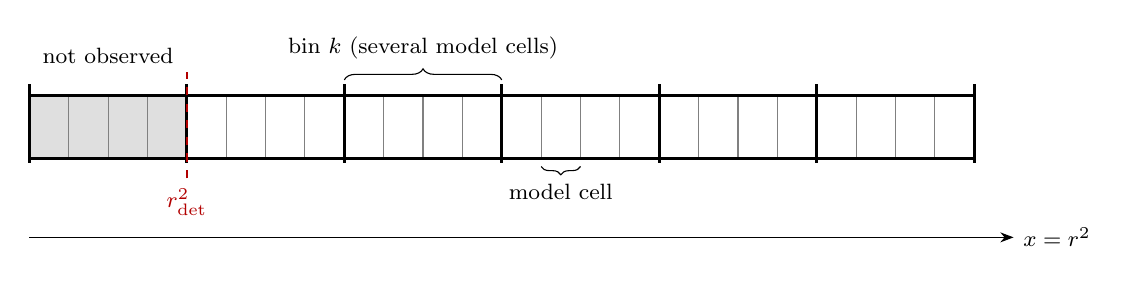
\begin{tikzpicture}[x=0.5cm,y=1cm,font=\footnotesize]
\fill[gray!25] (0,0) rectangle (4,0.8);
\foreach \i in {0,...,23}{\draw[gray] (\i,0) rectangle ++(1,0.8);}
\foreach \j in {0,4,8,12,16,20,24}{\draw[very thick] (\j,-0.05) -- (\j,0.95);}
\draw[very thick] (0,0) -- (24,0); \draw[very thick] (0,0.8) -- (24,0.8);
\node at (2,1.3) {not observed};
\draw[decorate,decoration={brace,amplitude=4pt}] (8,1.0) -- (12,1.0) node[midway,above=4pt] {bin $k$ (several model cells)};
\draw[decorate,decoration={brace,amplitude=3pt,mirror}] (13,-0.1) -- (14,-0.1) node[midway,below=3pt] {model cell};
\draw[red!70!black,dashed,thick] (4,-0.25) -- (4,1.1);
\node[red!70!black] at (4,-0.55) {$\rdet^2$};
\draw[-{Stealth}] (0,-1.0) -- (25,-1.0) node[right] {$x = r^2$};
\end{tikzpicture}\\[0.3em]
\raggedright
\small Bins below the detection limit are \textbf{unobserved, not zero}: there are plenty of droplets there; we just did not see them. They are left out of the fit. (Recording zeros would push $D_x$ toward suppressing small droplets.)
\end{frame}

%------------------------------------------------------------------
\begin{frame}{Expected counts $\mu_k$ and observed counts $c_k$}
\begin{columns}[T]
\begin{column}{0.5\textwidth}
\small\textbf{Well-mixed:} every part of the chamber holds the same distribution on average, so
\[
\mu_k = V\!\int_{\text{bin }k}\! N(x)\,dx
\]
\end{column}
\begin{column}{0.48\textwidth}
\small Each droplet is in the sample independently, with small probability $q = V/V_{\rm chamber}$:
\[
c_k \sim \mathrm{Poisson}(\mu_k),\qquad \mathrm{Var}\,c_k = \mu_k
\]
\end{column}
\end{columns}
\centering
\vspace{-0.6em}
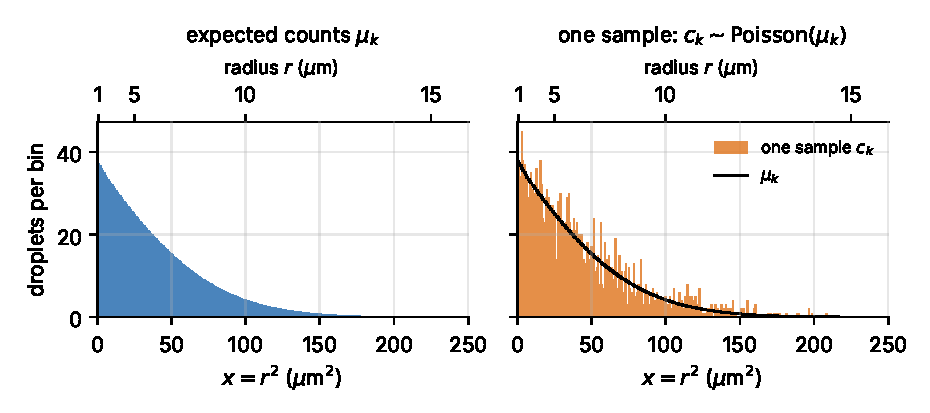
\includegraphics[width=0.68\textwidth]{d_mu_c.pdf}\\[-0.2em]
{\footnotesize $D_x = 10$, $V=0.1$ cm$^3$ ($\approx2000$ droplets), bins of $0.9\um^2$. The busiest bin expects 38 droplets; relative noise is $1/\sqrt{\mu_k}$.}
\end{frame}

%------------------------------------------------------------------
\begin{frame}{The number of droplets sets the noise}
\centering
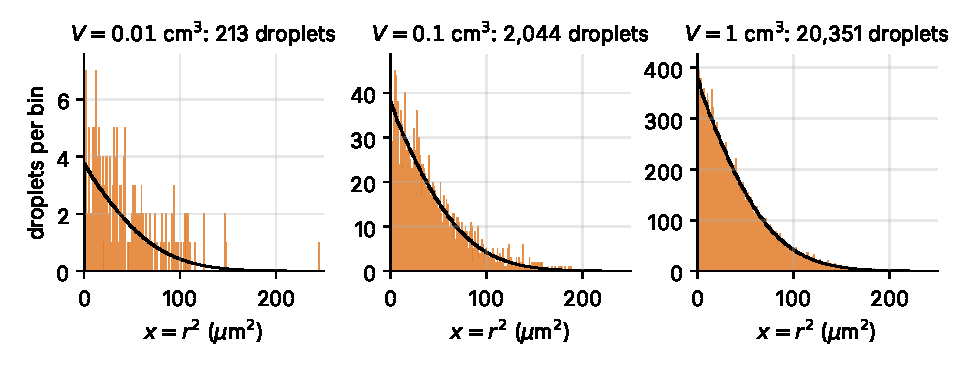
\includegraphics[width=0.95\textwidth]{d_samples.pdf}\\[0.3em]
\small One sample (orange) at each volume against the expected counts (black). Well-mixed removes \emph{bias}; it does not remove luck-of-the-draw \emph{noise}.
\end{frame}

%------------------------------------------------------------------
\begin{frame}{Loss function: from likelihood to Poisson deviance}
Independent Poisson counts give the likelihood of the observed histogram, a function of $\ell = \ln D_x$:
\[
L(\ell) = \prod_{k\,\in\,\text{obs}}\frac{\mu_k(\ell)^{c_k}\,e^{-\mu_k(\ell)}}{c_k!}
\qquad\Longrightarrow\qquad
-\ln L(\ell) = \sum_{k\,\in\,\text{obs}}\Bigl[\mu_k - c_k\ln\mu_k + \ln c_k!\Bigr]
\]
\begin{columns}[T]
\begin{column}{0.42\textwidth}
\textbf{Three changes} (none moves the minimum):
\begin{enumerate}
\item Drop $\ln c_k!$: it does not depend on $D_x$
\item Subtract its best possible value (at $\mu_k = c_k$), so a perfect fit scores 0
\item Multiply by 2
\end{enumerate}
\end{column}
\begin{column}{0.56\textwidth}
\begin{block}{Poisson deviance}
\vspace{-0.5em}
\[
\J(\ell) = 2\sum_{k\,\in\,\text{obs}}\Bigl[\,c_k\ln\frac{c_k}{\mu_k} \;-\; c_k \;+\; \mu_k\Bigr]
\]
\end{block}
\small
\begin{itemize}
\item For large counts, $\J\approx\sum_k (c_k-\mu_k)^2/\mu_k$: least squares with each bin weighted by its own noise
\item Plain least squares would let the busy peak bins dominate and nearly ignore the sparse tail
\end{itemize}
\end{column}
\end{columns}
\end{frame}

%==================================================================
\section{Estimation}
%==================================================================

\begin{frame}{Deriving the adjoint gradient}
\small
The loss depends on $D_x$ only through the model solution: $\J = \J\bigl(\N(D_x)\bigr)$, where $\A(D_x)\,\N = \mathbf{b}$.
\begin{columns}[T]
\begin{column}{0.5\textwidth}
\textbf{1. Chain rule}
\[
\frac{d\J}{dD_x} = \mathbf{g}^{\!\top}\frac{d\N}{dD_x},\qquad \mathbf{g} = \frac{\partial\J}{\partial\N}
\]
\textbf{2. Differentiate the model} ($\mathbf{b}$ does not depend on $D_x$)
\[
\frac{\partial\A}{\partial D_x}\N + \A\,\frac{d\N}{dD_x} = \mathbf{0}
\;\Rightarrow\;
\frac{d\N}{dD_x} = -\A^{-1}\frac{\partial\A}{\partial D_x}\N
\]
Computing $d\N/dD_x$ directly costs one solve per parameter.\\[0.4em]
\textbf{3. Substitute}
\[
\frac{d\J}{dD_x} = \underbrace{-\mathbf{g}^{\!\top}\A^{-1}}_{\bm\psi^{\!\top}}\;\frac{\partial\A}{\partial D_x}\N
\]
\end{column}
\begin{column}{0.48\textwidth}
\textbf{4. Solve for $\bm\psi$ instead.} The row vector $\bm\psi^{\!\top} = -\mathbf{g}^{\!\top}\A^{-1}$ does not depend on which parameter we differentiate:
\[
\bm\psi^{\!\top}\A = -\mathbf{g}^{\!\top}\quad\Longleftrightarrow\quad \A^{\!\top}\bm\psi = -\mathbf{g}
\]
\textbf{5. Gradient}
\[
\frac{d\J}{dD_x} = \bm\psi^{\!\top}\frac{\partial\A}{\partial D_x}\N,\qquad \frac{d\J}{d\ell} = D_x\,\frac{d\J}{dD_x}
\]
\textbf{Ingredients}
\begin{itemize}
\item From the loss, with $\bm\mu = V\mathsf{H}\N$: $\;\mathbf{g} = V\mathsf{H}^{\!\top}\bigl[2(1 - c_k/\mu_k)\bigr]$
\item $\partial\A/\partial D_x$: differentiate the flux coefficients; same tridiagonal pattern as $\A$
\end{itemize}
\end{column}
\end{columns}
\end{frame}

%------------------------------------------------------------------
\begin{frame}{The adjoint in practice}
\begin{columns}[T]
\begin{column}{0.52\textwidth}
\textbf{Each evaluation of loss and gradient}
\begin{enumerate}
\item Forward solve $\A\N = \mathbf{b}$ (LU factorization)
\item Loss $\J$ and $\mathbf{g} = \partial\J/\partial\N$
\item Adjoint solve $\A^{\!\top}\bm\psi = -\mathbf{g}$, reusing the same LU factors
\item Gradient $\bm\psi^{\!\top}(\partial\A/\partial D_x)\N$
\end{enumerate}
\vspace{0.4em}
\textbf{What $\bm\psi$ means.} Adding a small source $\delta\mathbf{b}$ of droplets changes the loss by
\[
\delta\J = -\bm\psi^{\!\top}\delta\mathbf{b},
\]
so $\psi_i>0$ where adding droplets would \emph{improve} the fit.
\end{column}
\begin{column}{0.46\textwidth}
\centering
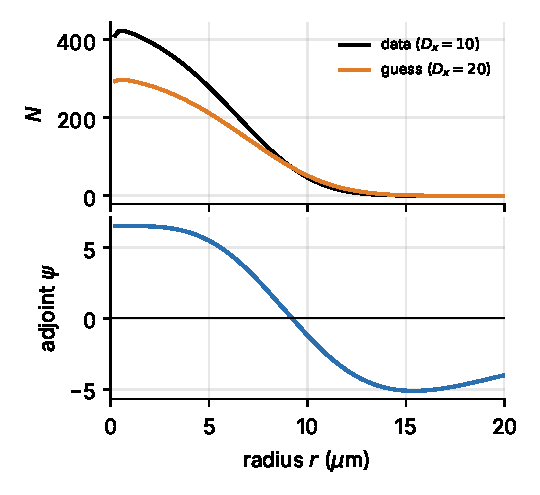
\includegraphics[width=0.92\textwidth]{d_adjoint_stack.pdf}\\
{\footnotesize At $D_x = 20$ the model is short of small and mid-sized droplets ($\psi>0$) and has too many large ones ($\psi<0$).}
\end{column}
\end{columns}
\end{frame}

%------------------------------------------------------------------
\begin{frame}{Why the adjoint?}
\begin{columns}[T]
\begin{column}{0.54\textwidth}
\small
\begin{tabular}{@{}lc@{}}
\toprule
Gradient method & cost for $P$ parameters\\\midrule
Finite differences & $2P$ forward solves\\
Forward sensitivities & $P$ extra solves\\
\textbf{Adjoint} & \textbf{1 extra solve, any $P$}\\\bottomrule
\end{tabular}\\[0.6em]
\normalsize
\begin{itemize}
\item The adjoint solve reuses the factorization of $\A$, so it is cheap
\item Exact gradient of the computed loss
\item With one parameter it is not \emph{needed}. It is an investment: $s$, injection rate, an unknown initial distribution, or a time-varying $s(t)$ add many unknowns but no extra cost
\end{itemize}
\end{column}
\begin{column}{0.44\textwidth}
\textbf{Optimizer}
\begin{itemize}
\item Gradient descent in $\ell = \ln D_x$
\item Step size from the last two gradients
\item At most a factor $e$ change per iteration
\item Backtrack until the loss decreases
\end{itemize}
\end{column}
\end{columns}
\end{frame}

%------------------------------------------------------------------
\begin{frame}{An error bar from a single sample}
\begin{columns}[T]
\begin{column}{0.48\textwidth}
\begin{itemize}
\item Real data come as \textbf{one} sample, so we need an error bar from that sample alone
\item Near its minimum the loss is a parabola, and $\J = -2\ln L + {}$const, so the likelihood is Gaussian in $\ell$:
\[
\mathrm{sd}(\hat\ell) \approx \sqrt{2/\J''(\hat\ell)}
\]
\item $\J''$: finite difference of the adjoint gradient
\item $\ell = \ln D_x$, so this is a \emph{relative} error
\item Predicted in advance by the Fisher information $\mathcal I = \sum_k (\partial_\ell\mu_k)^2/\mu_k \propto V$
\end{itemize}
\end{column}
\begin{column}{0.5\textwidth}
\centering
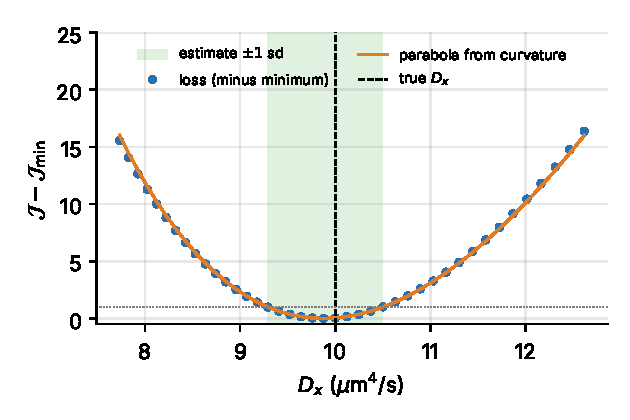
\includegraphics[width=\textwidth]{d_single.pdf}\\
{\footnotesize One sample, true $D_x = 10$, $\approx2000$ droplets: $\hat D_x = 9.88$, sd $= 6\%$, interval $[9.3, 10.5]$.}
\end{column}
\end{columns}
\end{frame}

%==================================================================
\section{Results}
%==================================================================

\begin{frame}{Sanity check: exact data}
\centering
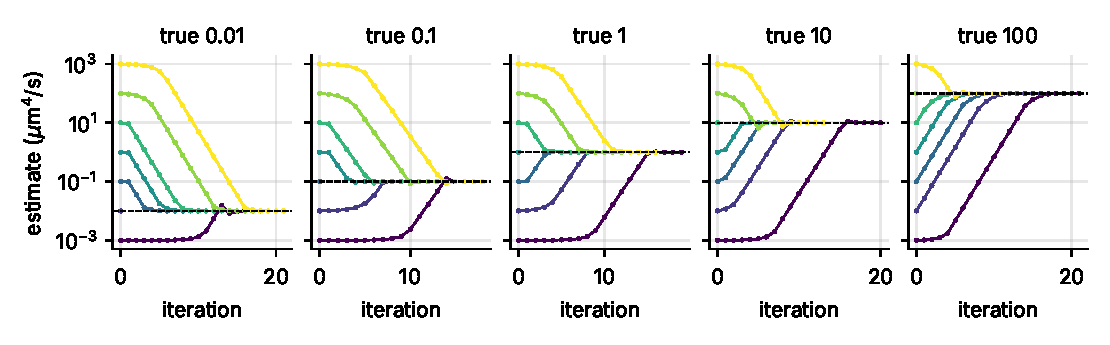
\includegraphics[width=\textwidth]{d_sweep.pdf}\\[0.2em]
\begin{itemize}\small
\item 5 true values $\times$ 7 starting guesses ($10^{-3}$, dark, to $10^{3}\um^4$/s, yellow): all recovered to a relative error $<5\times10^{-9}$, in at most 21 iterations
\item Starting guesses $\le 10^{-4}$ fail: below the numerical-diffusion floor the gradient vanishes
\end{itemize}
\end{frame}

%------------------------------------------------------------------
\begin{frame}{Precision versus number of droplets}
\begin{columns}[T]
\begin{column}{0.46\textwidth}
\centering
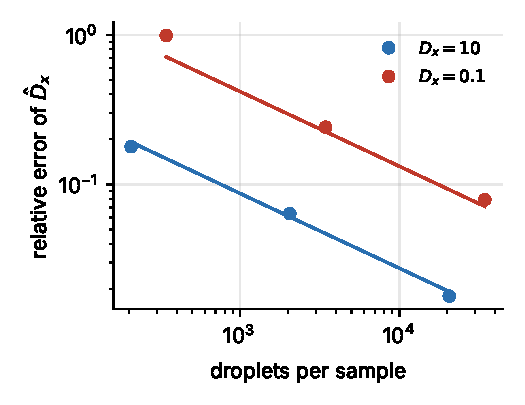
\includegraphics[width=\textwidth]{d_scaling.pdf}\\
{\footnotesize Spread of $\hat D_x$ over 200 independent samples (dots) vs.\ prediction $1/\sqrt{\mathcal I}$ (lines).}
\end{column}
\begin{column}{0.52\textwidth}
\begin{itemize}
\item Estimates are unbiased
\item Error $\propto 1/\sqrt{\text{droplets}}$. For $D_x = 10$: $19\%$, $6\%$, $2\%$ with about 200, 2000, 20{,}000 droplets
\item $D_x = 0.1$ is about $5\times$ harder for the same number of droplets
\item With very little information (error $\gtrsim50\%$) estimates skew low and the prediction is optimistic
\end{itemize}
\end{column}
\end{columns}
\end{frame}

%------------------------------------------------------------------
\begin{frame}{Single-sample error bars are honest}
\centering
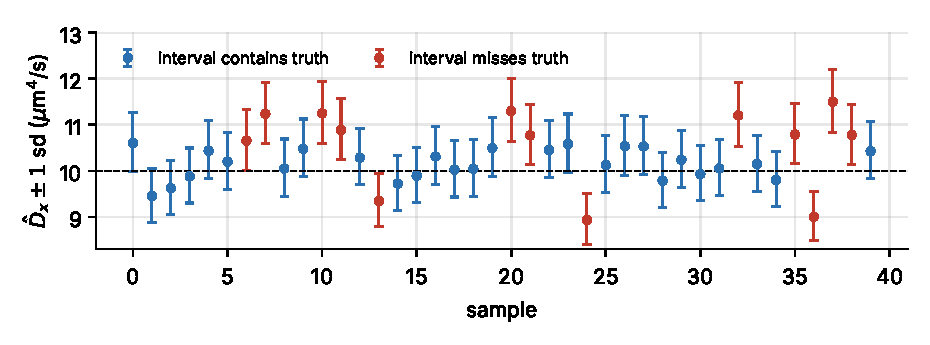
\includegraphics[width=0.76\textwidth]{d_errorbars.pdf}\\[-0.1em]
{\footnotesize First 40 samples, true $D_x=10$, about 2000 droplets each: 27 of 40 intervals contain the truth.}\\[0.3em]
\small
\begin{tabular}{@{}lcccccc@{}}
\toprule
$D_x$ & \multicolumn{3}{c}{10} & \multicolumn{3}{c}{0.1}\\
\cmidrule(lr){2-4}\cmidrule(lr){5-7}
droplets per sample & 200 & 2000 & 20{,}000 & 340 & 3400 & 34{,}000\\\midrule
truth within $\pm1$ sd (ideal 68\%) & 71\% & 69\% & 72\% & 67\% & 62\% & 64\%\\
truth within $\pm2$ sd (ideal 95\%) & 97\% & 93\% & 97\% & 95\% & 94\% & 91\%\\\bottomrule
\end{tabular}
\end{frame}

%------------------------------------------------------------------
\begin{frame}{Why is large $D_x$ easier to recover?}
\begin{columns}[T]
\begin{column}{0.47\textwidth}
\centering
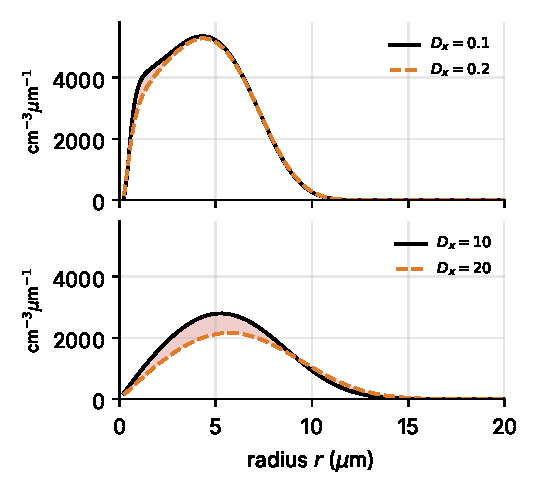
\includegraphics[width=0.95\textwidth]{d_doubling_stack.pdf}\\
{\footnotesize Doubling $D_x$ changes the distribution by 4\% at $D_x=0.1$ (top), 22\% at $D_x = 10$ (bottom).}
\end{column}
\begin{column}{0.51\textwidth}
\begin{itemize}\small
\item Not breadth itself: the \textbf{share of the width caused by $D_x$}
\item Even with no turbulence the distribution is broad: droplets of many different ages coexist. $D_x$ only adds to that
\item Small $D_x$ adds very little, so the data barely respond to it
\item Physics, not numerics: information per droplet at $D_x=0.1$ is unchanged on a $4\times$ finer grid
\item Relative vs.\ absolute: with 2000 droplets, $0.1\pm0.024$ vs.\ $10\pm0.6$
\end{itemize}
\vspace{0.3em}
\centering\footnotesize
\begin{tabular}{@{}lcccc@{}}
\toprule
$D_x$ ($\mu$m$^4$/s) & 0.1 & 1 & 10 & 100\\\midrule
share of width from $D_x$ & 2.5\% & 18\% & 48\% & 62\%\\
pred.\ error (2000 drops) & 24\% & 15\% & 6\% & 5\%\\\bottomrule
\end{tabular}
\end{column}
\end{columns}
\end{frame}

%------------------------------------------------------------------
\begin{frame}{Detection limit: harmless for large $D_x$, severe for small}
\begin{columns}[T]
\begin{column}{0.46\textwidth}
\centering
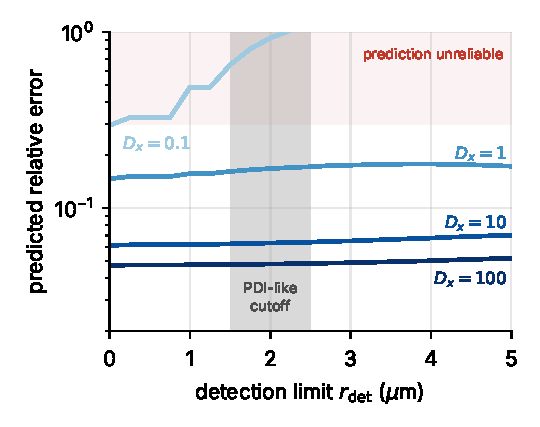
\includegraphics[width=\textwidth]{d_cutoff_pred.pdf}\\
{\footnotesize Predicted error with 2000 droplets counted above the cutoff.}
\end{column}
\begin{column}{0.52\textwidth}
\small
Monte Carlo, 200 samples each (relative error of $\hat D_x$):\\[0.3em]
\begin{tabular}{@{}lcc@{}}
\toprule
& $D_x=10$ & $D_x=0.1$\\
cutoff $\rdet$ & 2000 droplets & 34{,}000 droplets\\\midrule
none & 6.4\% & 7.9\%\\
$1\um$ & 6.0\% & 12\%\\
$2\um$ & 6.9\% & 27\%\\
$3\um$ & 7.0\% & 56\%\\\bottomrule
\end{tabular}
\begin{itemize}
\item Large $D_x$: its fingerprint is spread over the whole distribution
\item Small $D_x$: its fingerprint is near activation, $r\approx1$--$2\um$, exactly what a cutoff hides
\end{itemize}
\end{column}
\end{columns}
\end{frame}

%==================================================================
\section{Takeaways and next steps}
%==================================================================

\begin{frame}{Takeaways and caveats}
\begin{columns}[T]
\begin{column}{0.5\textwidth}
\textbf{Takeaways}
\begin{itemize}
\item Exact data: $D_x$ recovered from any reasonable starting guess (above the grid's numerical-diffusion floor)
\item Counts: unbiased estimates, error $\propto1/\sqrt{\text{droplets}}$
\item A single sample's curvature error bar is trustworthy
\item Large $D_x$ is easy; small $D_x$ is hard because turbulence is a small share of the width
\item The detection limit matters mainly for small $D_x$
\end{itemize}
\end{column}
\begin{column}{0.48\textwidth}
\textbf{Caveats}
\begin{itemize}
\item \emph{Inverse crime}: data generated by the same model and grid that we fit
\item Poisson assumes independent sampling; real counts may vary more (clustering, a fluctuating chamber-wide $s$)
\item $D_x$ is \emph{effective}: any unmodeled broadening (sizing error, fluctuating $s$, wall effects) gets absorbed into it
\item The well-mixed assumption is weakest for large, fast-falling droplets
\end{itemize}
\end{column}
\end{columns}
\end{frame}

%------------------------------------------------------------------
\begin{frame}{Next steps}
\begin{enumerate}
\item \textbf{Drift and diffusion together:} estimate $s$ with $D_x$. Both affect the width; $s$ also sets the scale. Can a steady distribution separate them? (Note $a$ and $s$ enter as the product $a\,s$.)
\item \textbf{Remove the inverse crime:} generate the truth on a finer grid than the fit
\item \textbf{Stochastic particle model:} finite numbers of droplets with the same physics, as a stand-in for Lagrangian simulation data
\item \textbf{Simulation output:} C-ODT, then bin LES, super-droplet LES, DNS. Compare fitted $D_x$ with $a^2\sigma_s^2\tau_s$ measured along droplet paths
\item \textbf{Chamber data}, then time dependence
\end{enumerate}
\end{frame}

%==================================================================
\section{Questions for the MTU group}
%==================================================================

\begin{frame}{Q1. What is the volume ratio $q = V/V_{\rm chamber}$?}
\begin{columns}[T]
\begin{column}{0.46\textwidth}
\textbf{What we assume}
\begin{itemize}
\item Poisson counts need each droplet to land in the sample independently, with $q \ll 1$
\item Pi Chamber $\approx3$ m$^3$, samples of $0.01$--$1$ cm$^3$: $q\approx3\times10^{-9}$--$3\times10^{-7}$
\item Simulations that report every droplet have $q = 1$: no sampling noise at all
\end{itemize}
\end{column}
\begin{column}{0.52\textwidth}
\ask{What we'd like to know}
\begin{itemize}
\item What effective volume is behind one histogram? (PDI: probe area $\times$ flow speed $\times$ averaging time?)
\item Do successive histograms recount the same droplets? Droplets live for minutes.
\item In simulations, how much does the whole-domain distribution fluctuate between snapshots of a steady run?
\end{itemize}
\end{column}
\end{columns}
\end{frame}

%------------------------------------------------------------------
\begin{frame}{Q2. How many droplets are in a sample?}
\begin{columns}[T]
\begin{column}{0.5\textwidth}
Predicted error in $\hat D_x$, detection limit $2.5\um$:\\[0.4em]
\begin{tabular}{@{}rccc@{}}
\toprule
& \multicolumn{3}{c}{droplets counted}\\
\cmidrule(lr){2-4}
$D_x$ ($\mu$m$^4$/s) & 200 & 2000 & 20{,}000\\\midrule
100 & 15\% & 5\% & 1.5\%\\
10 & 20\% & 6\% & 2\%\\
1 & 54\% & 17\% & 5\%\\
0.1 & $>100\%$ & $>100\%$ & 35\%\\\bottomrule
\end{tabular}\\[0.3em]
{\footnotesize From the Fisher information; reliable below about 30\%.}
\end{column}
\begin{column}{0.48\textwidth}
\textbf{Our setup:} the model's concentration ($\approx2\times10^4$ cm$^{-3}$) comes from an arbitrary injection rate.\\[0.6em]
\ask{What we'd like to know}
\begin{itemize}
\item Typical droplet concentration, and droplets per histogram
\item Averaging time per histogram; how many independent histograms per steady state
\item A realistic activation rate for the model
\end{itemize}
\end{column}
\end{columns}
\end{frame}

%------------------------------------------------------------------
\begin{frame}{Q3. What are realistic values of $D_x$?}
\begin{columns}[T]
\begin{column}{0.52\textwidth}
Our reading of the stochastic theory (Chandrakar et al.\ 2016, 2018):
\[
D_x = a^2\sigma_s^2\tau_s = \frac{a^2\,\sigma_{s_0}^2\,\tau_t}{(1+\mathrm{Da})^2},\qquad a = 2\xi
\]
With their fitted $\tau_t\approx40$--$48$ s and $\sigma_{s_0}$, in $\mu$m$^4$/s:\\[0.3em]
\begin{tabular}{@{}lcccc@{}}
\toprule
& Da $=0.3$ & 1 & 5 & 40\\\midrule
$\Delta T = 16$ K & 40 & 18 & 2 & --\\
$\Delta T = 19$ K & 260 & 110 & 12 & 0.3\\\bottomrule
\end{tabular}\\[0.3em]
$\Rightarrow$ roughly $1$--$200\um^4$/s.
\end{column}
\begin{column}{0.46\textwidth}
\ask{What we'd like to know}
\begin{itemize}
\item Is this mapping to $D_x$ right?
\item Can DNS/LES give supersaturation statistics along droplet paths ($\sigma_s$, $\tau_s$), for a direct check?
\item With $\tau_t\approx40$--$50$ s and growth times of minutes, is a constant diffusivity adequate?
\end{itemize}
\end{column}
\end{columns}
\end{frame}

%------------------------------------------------------------------
\begin{frame}{Q4. What is the detection limit?}
\begin{columns}[T]
\begin{column}{0.47\textwidth}
\centering
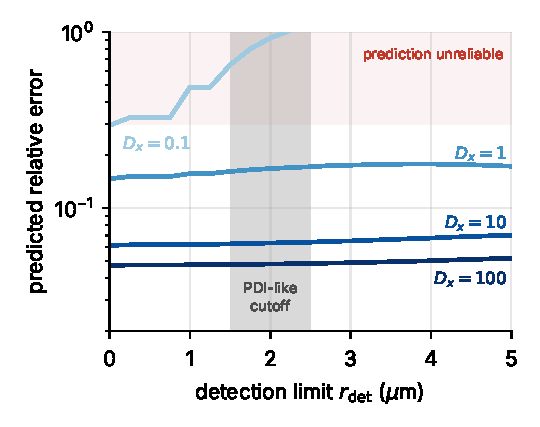
\includegraphics[width=\textwidth]{d_cutoff_pred.pdf}\\
{\footnotesize Predicted error with 2000 droplets counted above the cutoff.}
\end{column}
\begin{column}{0.51\textwidth}
Chandrakar et al.\ (2018), phase Doppler: kept diameters $\ge5\um$, i.e.\ $\rdet\approx2.5\um$.
\begin{itemize}
\item $D_x\gtrsim1$: the cutoff costs little
\item $D_x\lesssim0.1$: its fingerprint is near activation ($1$--$2\um$) and is lost
\end{itemize}
\ask{What we'd like to know}
\begin{itemize}
\item Which instruments and cutoffs apply now?
\item Detection efficiency vs.\ size near the cutoff?
\item Sizing uncertainty and bin edges?
\end{itemize}
\end{column}
\end{columns}
\end{frame}

%------------------------------------------------------------------
\begin{frame}{Q5 and Q6. What else shapes the measured distribution?}
\begin{columns}[T]
\begin{column}{0.49\textwidth}
\ask{Q5. What else broadens it?}\\[0.3em]
Anything missing from the model is absorbed into the fitted $D_x$:
\begin{itemize}
\item Instrument sizing error
\item Slow fluctuations of the chamber-wide $s$ (large-scale circulation, oscillation)
\item Subsaturated wall regions; large droplets concentrated near the floor
\item Polydisperse aerosol; coalescence in the tail
\end{itemize}
Which of these matter most in the chamber, and how large are they?
\end{column}
\begin{column}{0.49\textwidth}
\ask{Q6. Can the mean supersaturation be measured?}\\[0.3em]
\begin{itemize}
\item $s$ also affects the width (higher $s$: droplets grow larger before falling out), so a wrong $s$ biases $D_x$
\item Our next step estimates $s$ and $D_x$ together
\item Is $s$ known from temperature and humidity measurements, diagnosed from LES, or must it be inferred?
\item How steady is $s$ over the time one histogram takes?
\end{itemize}
\end{column}
\end{columns}
\end{frame}

%------------------------------------------------------------------
\begin{frame}{Summary of asks}
\begin{enumerate}
\item \ask{Volume ratio $q$:} effective volume per histogram; are successive histograms independent?
\item \ask{Droplets per sample:} concentrations, droplets per histogram, averaging time
\item \ask{Realistic $D_x$:} is $D_x = a^2\sigma_s^2\tau_s$ right; supersaturation statistics along droplet paths
\item \ask{Detection limit:} cutoff, efficiency curve, sizing uncertainty
\item \ask{Other broadening:} which unmodeled effects matter, and how much
\item \ask{Mean supersaturation:} measured, diagnosed, or estimated?
\end{enumerate}
\vspace{0.5em}
\textbf{Most useful simulation data:} whole-domain size distributions (or droplet lists with multiplicities) from statistically steady runs, with the run configuration ($\Delta T$, injection rate, aerosol size, chamber height).
\end{frame}

%==================================================================
\appendix
\begin{frame}[standout]
Backup
\end{frame}

%------------------------------------------------------------------
\begin{frame}{Backup: why the counts are Poisson}
A bin holding $M$ droplets; each is in the sample independently with probability $q = V/V_{\rm chamber}$:
\[
P(c) = \binom{M}{c}q^c(1-q)^{M-c}
= \underbrace{\frac{M\cdots(M-c+1)}{M^c}}_{\to1}\,\frac{\mu^c}{c!}\,\underbrace{\Bigl(1-\frac{\mu}{M}\Bigr)^{M}}_{\to e^{-\mu}}\underbrace{\Bigl(1-\frac{\mu}{M}\Bigr)^{-c}}_{\to1}
\;\longrightarrow\;\frac{\mu^c e^{-\mu}}{c!}
\]
as $M\to\infty$, $q\to0$ with $\mu = Mq$ fixed.
\begin{itemize}
\item Bins are independent: a Poisson total split independently among bins gives independent Poisson bins
\item Neighboring bins have similar \emph{expected} counts (the model handles that); independence is about their \emph{errors}
\item Not covered: clustering, a fluctuating chamber-wide $s$, an uncertain $V$. These correlate bins and make counts more variable than Poisson.
\end{itemize}
\end{frame}

%------------------------------------------------------------------
\begin{frame}{Backup: the Scharfetter--Gummel flux}
Between neighboring cell centers, treat $A$ and $F$ as constant. Then $D_x N' = AN - F$ is a linear ODE with solution $N = F/A + C e^{A(x-x_i)/D_x}$. Matching $N_i$ and $N_{i+1}$ gives
\[
F_{i+1/2} = \frac{D_x}{\Delta x}\Bigl[B(-\mathrm{Pe}_i)\,N_i - B(\mathrm{Pe}_i)\,N_{i+1}\Bigr],\qquad
\mathrm{Pe}_i = \frac{A_{i+1/2}\Delta x}{D_x},\quad B(z) = \frac{z}{e^z-1}
\]
\begin{itemize}
\item $|\mathrm{Pe}|\ll1$: ordinary diffusion plus drift times the average of $N_i, N_{i+1}$
\item $\mathrm{Pe}\gg1$: $F\to A\,N_i$, the upstream value; never negative
\item Equivalent to central differencing with $D_{\rm eff} = D_x\,\tfrac{\mathrm{Pe}}{2}\coth\tfrac{\mathrm{Pe}}{2}\ge D_x$; for large Pe, $D_{\rm eff}\to|A|\Delta x/2$, independent of $D_x$
\end{itemize}
\end{frame}

\end{document}
